\documentclass[10pt,utf8]{beamer}

\mode<presentation> {
  \usetheme{Madrid}
  \setbeamercovered{transparent}
}

\usepackage{palatino}
\usepackage{graphicx}
\usepackage{array}
\usepackage{color}
\usepackage{subfigure}
\usepackage{colortbl}
\usepackage{amsmath}
\usepackage{hyperref}
\usepackage{listings}
\usepackage{fancyvrb}

\setbeamertemplate{caption}{\raggedright\insertcaption\par} %turn off caption prefix ("Figure")

\definecolor{delim}{RGB}{20,105,176}
\definecolor{numb}{RGB}{106, 109, 32}
\definecolor{string}{rgb}{0.64,0.08,0.08}

\lstdefinestyle{java}{
	basicstyle          = \normalsize\ttfamily,
	language            = java,
	numbers             = left,
	numberstyle         = \small,
	stepnumber          = 1,
	numbersep           = 5pt,
	backgroundcolor     = \color{white},
	showspaces          = false,
	showstringspaces    = false,
	showtabs            = false,
	frame               = single,
	tabsize             = 2,
	captionpos          = b,
	breaklines          = true,
	breakatwhitespace   = false,
	morestring          = [b]",
	stringstyle         = \color{blue},
	keywordstyle        = \color{magenta},
	commentstyle        = \color{gray},
	identifierstyle     = \color{black},
	moredelim           = **[is][\bfseries]{`}{`},
	moredelim           = **[is][\color{magenta}]{$}{$}, 
	fancyvrb            = true,
}


\title{Debezium Asynchronous Engine}
\author{Vojtěch Juránek}
\institute[Red Hat]{Red Hat}
\date{May 21st 2024, Debezium F2F meeting, Brno}

\newenvironment{mylisting}
{\begin{list}{}{\setlength{\leftmargin}{1em}}\item\scriptsize\bfseries}
{\end{list}}

\newenvironment{mytinylisting}
{\begin{list}{}{\setlength{\leftmargin}{1em}}\item\tiny\bfseries}
{\end{list}}


\begin{document}

\begin{frame}
    \titlepage
\end{frame}

\begin{frame}
    \frametitle{Debezium embedded engine}
    \begin{figure}
        \centering
        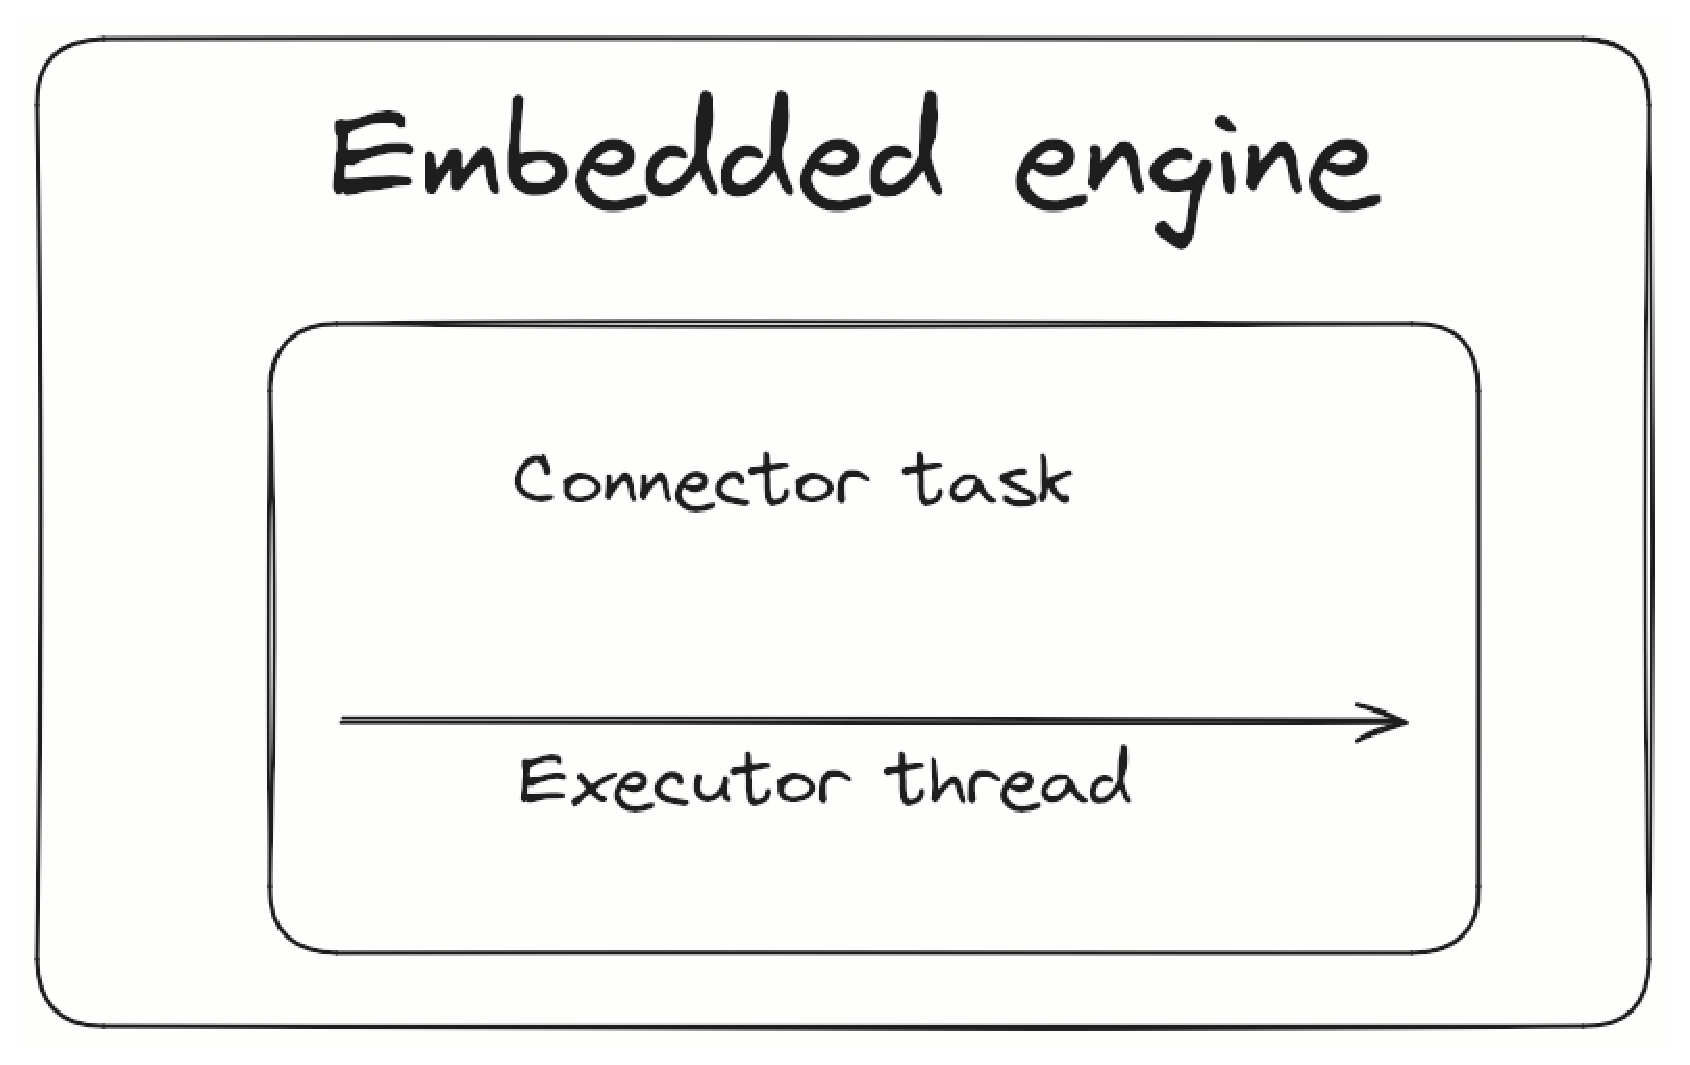
\includegraphics[height=6cm]{./img/embedded_engine.eps}
    \end{figure}
\end{frame}

\begin{frame}
    \frametitle{Asynchronous engine goals}
    \begin{itemize}
        \item Allow to run multiple source tasks for given connector if the connector provides multiple tasks.
        \item Run potentially time-consuming code (e.g. event transformation or serialization) in the dedicated threads.
        \item Allow possible further speedup by optionally disabling total ordering of the messages.
        \item Be well-prepared for future changes and new features:
        \begin{itemize}
            \item Switch to virtual threads.
            \item Delegate tasks to external works using gRPC.
            \item Provide Debeziuum engine as a Quarkus extension.
            \item \dots
        \end{itemize}
        \item Adjust Debezium testsuite to use \texttt{DebeziumEngine} interface instead hardcoded \texttt{EmbeddedEngine}.
    \end{itemize}
\end{frame}

\begin{frame}
    \frametitle{Asynchronous engine non-goals}
    \begin{itemize}
        \item Change \texttt{DebeziumEngine} interface.
        \item Implement any parallelization inside connectors.
        \item Remove dependency on Kafka Connect API.
        \item Add support for multiple source connectors or sink connector.
    \end{itemize}
\end{frame}


\begin{frame}
    \frametitle{Debezium asynchronous engine}
    \begin{figure}
        \centering
        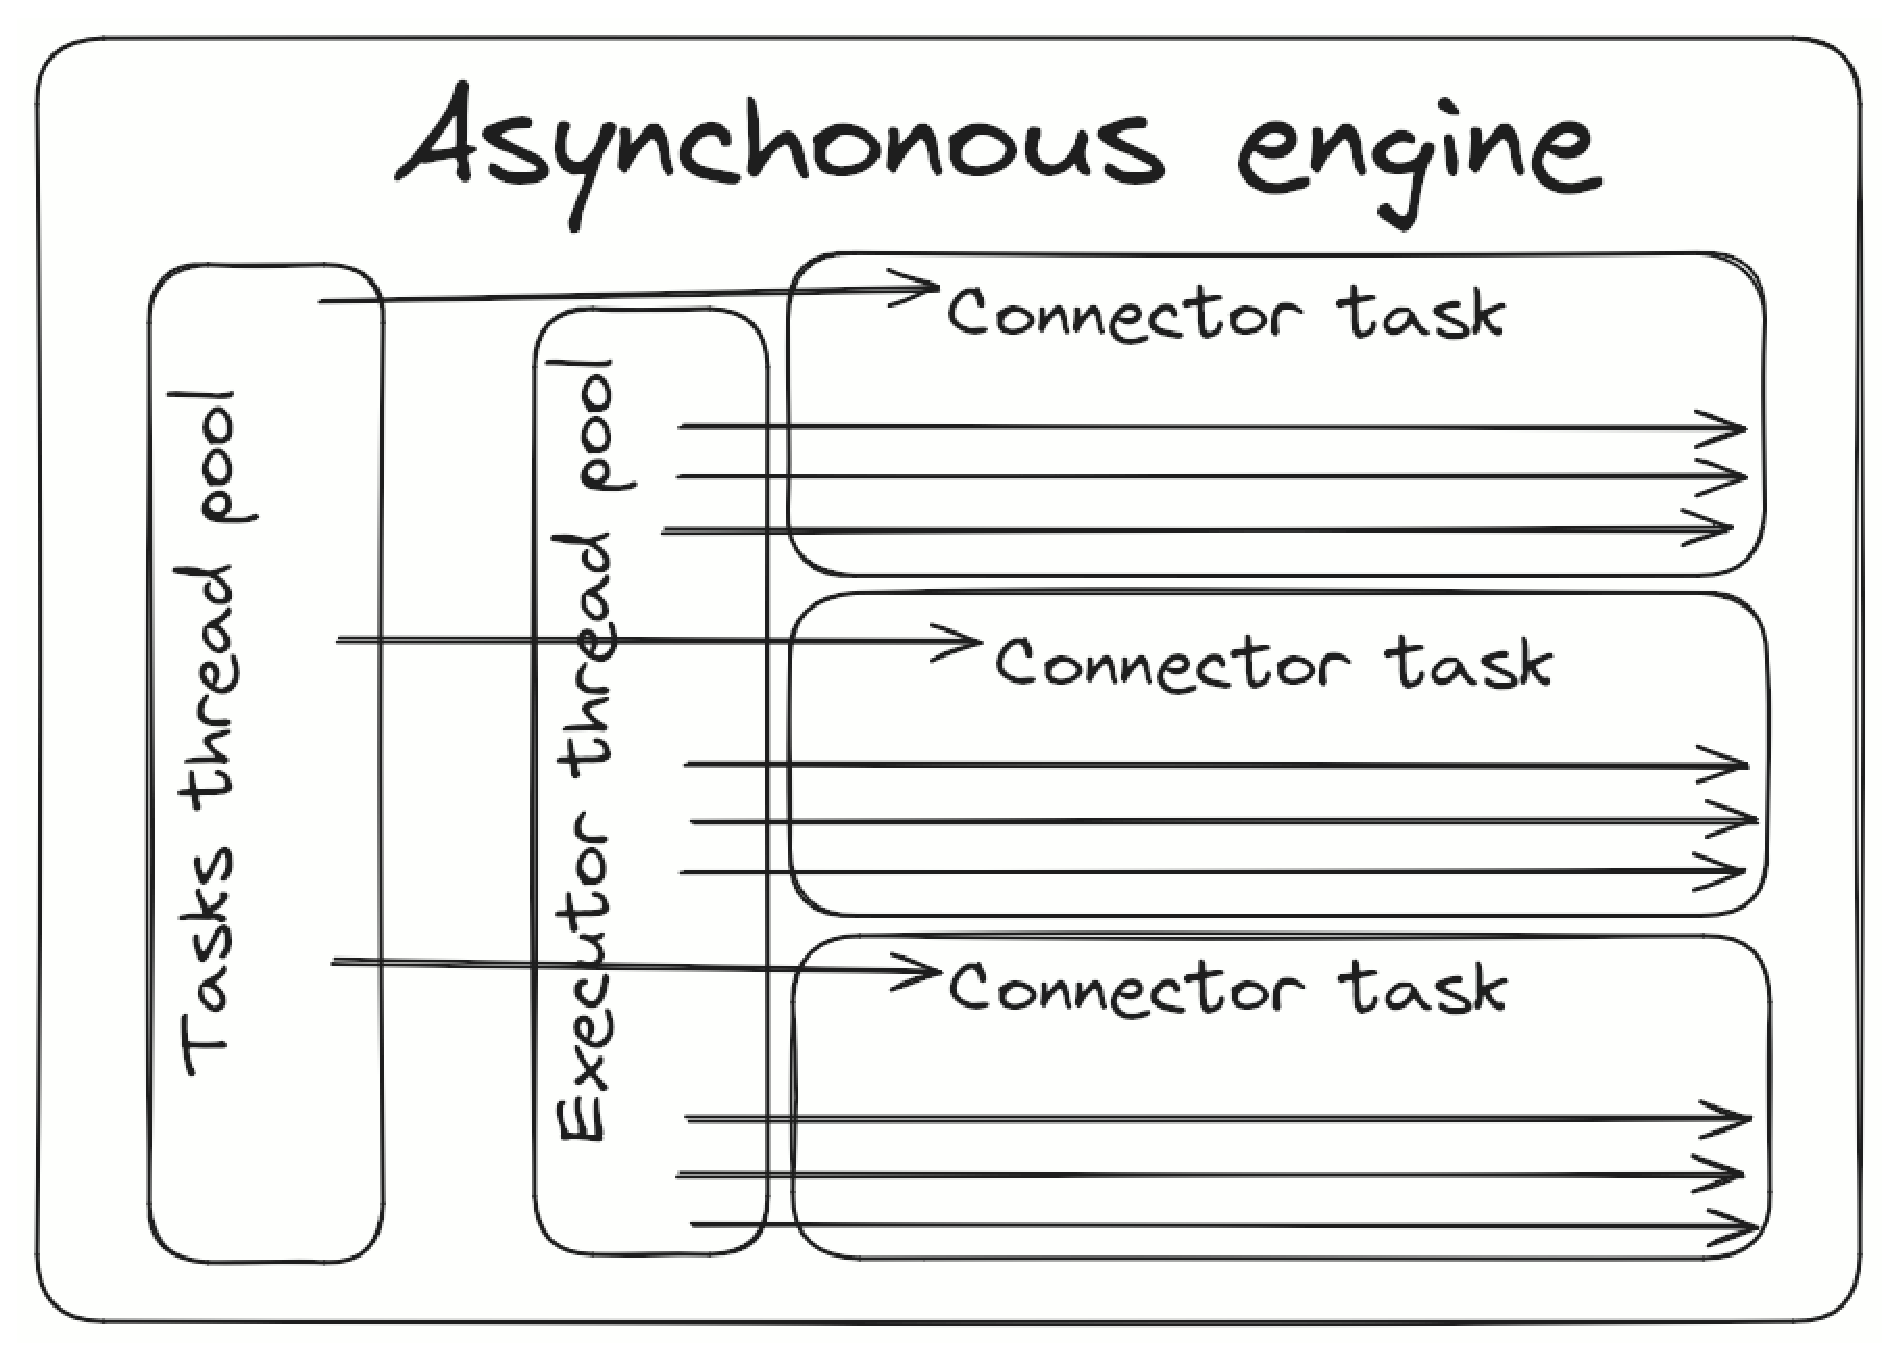
\includegraphics[height=6cm]{./img/async_engine.eps}
    \end{figure}
\end{frame}

\begin{frame}
    \frametitle{Engine states}
    \begin{itemize}
        \item \texttt{CREATING} - engine object is being created or was already created, but \texttt{run()} method wasn't called yet
        \item \texttt{INITIALIZING} - initializing the connector
        \item \texttt{CREATING\_TASKS} - creating connector tasks
        \item \texttt{STARTING\_TASKS} - starting connector tasks
        \item \texttt{POLLING\_TASKS} - running tasks polling, this is the main phase when the data are produced
        \item \texttt{STOPPING} - the engine is being stopped
        \item \texttt{STOPPED} - engine has been stopped, any call on engine object in this state should fail
    \end{itemize}
\end{frame}


\begin{frame}[fragile]
    \frametitle{Record processor}
    \begin{lstlisting}[style=java]
@Incubating
public interface RecordProcessor<R> {
    void initialize(
        final ExecutorService recordService,
        final Transformations transformations,
        final Function<SourceRecord, R> serializer,
        final RecordCommitter committer);

    void processRecords(final List<SourceRecord> records) throws InterruptedException;
}
    \end{lstlisting}
\end{frame}

\begin{frame}
    \frametitle{Async engine specific configuration options}
    \begin{itemize}
        \item \texttt{record.processing.threads} - number of threads to be used for processing CDC records.
        \item \texttt{record.processing.shutdown.timeout.ms} - maximum time in milliseconds to wait for processing submitted records when task shutdown is called.
        \item \texttt{record.processing.order} - determines how the records should be produced (\texttt{ORDERED}, \texttt{UNORDERED}).
        \item \texttt{record.processing.with.serial.consumer} - specifies whether the default ChangeConsumer should be created from provided Consumer, resulting in serial Consumer processing.
        \item \texttt{task.management.timeout.ms} - time to wait for task's lifecycle management operations (starting and stopping).
    \end{itemize}
\end{frame}

\begin{frame}
    \frametitle{Auxiliary interfaces and classes}
\end{frame}


\begin{frame}
    \frametitle{Future}
    \begin{itemize}
        \item gRPC
        \item virtual threads  - switching just few lines of code
    \end{itemize}
\end{frame}

\begin{frame}
    \frametitle{Resource}
    \begin{itemize}
        \color{blue}
        \item \href{https://github.com/debezium/debezium-design-documents/blob/main/DDD-7.md}{DDD-7: Asynchronous Debezium Embedded Engine}
        \item \href{https://github.com/debezium/debezium-design-documents/pull/8}{Discussion under DDD-7 PR}
        \color{black}
    \end{itemize}
\end{frame}


%%%%%%%%%%%%%%%%%%%%%%%%%%%%%%%%%%%%%%%%%%%%%%%%%%%%%%%%%%%%%%%%%%%%%%%%%%%%%%%%%%%%%%%%%%%%%%%%%
%%% BACKUP
%%%%%%%%%%%%%%%%%%%%%%%%%%%%%%%%%%%%%%%%%%%%%%%%%%%%%%%%%%%%%%%%%%%%%%%%%%%%%%%%%%%%%%%%%%%%%%%%%

% \begin{frame}
%     \centering
%     \huge{\textbf{Backup slides}}
% \end{frame}

\end{document}
